\documentclass[parskip=full]{scrartcl}

\usepackage[utf8]{inputenc}			% Umlaute, Sonderzeichen
\usepackage[ngerman]{babel}			% deutsche Sprache
%\usepackage[tocfullflat]{tocstyle}		% Inhaltsverzeichnis
\usepackage{enumitem}				% Listen
\usepackage{graphicx}					% Grafiken
\usepackage{hyperref}					% Hyperlinks
\usepackage[nonumberlist]{glossaries}		% Glossar

% Hurenkinder und Schusterjungen verhindern
\clubpenalty10000
\widowpenalty10000
\displaywidowpenalty=10000

\DeclareRobustCommand{\glossfirstformat}[1]{\textit{#1}}
\renewcommand*{\glsdisplayfirst}[4]{\glossfirstformat{#1#4}}

%\setcounter{tocdepth}{2}				% keine subsubsections im Inhaltsverzeichnis
\makenoidxglossaries     

\newglossaryentry{bsp}{
	name=Beispiel,
	plural=Beispiele,
	description=Beispieleintrag
	}

\newglossaryentry{UI}{
	name=UI,
	description={engl. User Interface. Steht für die Oberfläche, die der Benutzer verwendet um die Anwendung zu bedienen}
}

\newglossaryentry{RasPi}{
	name=Raspberry Pi,
	plural=Raspberry Pis,
	description={Der Raspberry Pi ist ein Einplatinencomputer. In diesem Projekt dient der Raspberry Pi als Hardwareplattform, um unterschiedliche Sensoren zu verbinden und ihre Daten auszulesen}
	}

\newglossaryentry{PhyPiDAQ}{
	name=PhyPiDAQ,
	description={Siehe Abschnitt 4.3 ,,PhyPiDAQ``}
	}

\newglossaryentry{Science Labs}{
	name=Science Labs,
	description={Ein Science Lab ist ein Arbeitsplatz, welcher Schülern ermöglicht wissenschaftliche Forschungen unter kontrollierten Bedingungen durchzuführen} 
	}

\newglossaryentry{Open-Source Projekt}{
	name=Open Source Projekt,
	description={Ein Open Source Projekt ist ein Projekt, dessen Quelltext und Dokumentationen von dritten angesehen, geändert und genutzt werden kann} 
	}

\newglossaryentry{OSL 2}{
	name=OSL 2,
	description={Name eines Open-Source-Lehrsoftware-Labor, in welchem Studierende sich mit der Entwicklung von Open-Source-Software vertraut machen können}
	}

\newglossaryentry{dragdrop}{
	name=Drag-and-Drop,
	description={Methode, um mit graphischen Benutzeroberflächen zu interagieren. Dabei wird ein Objekt erst mit der Maus festgehalten und an einen anderen Ort gezogen. Durch das Lösen der Maustaste wird das Objekt platziert}
	}

\newglossaryentry{click}{
	name=Click,
	description={Betätigen der linken Maustaste}
	}

\newglossaryentry{transformation}{
	name=Transformation,
	plural={Transformationen},
	description={Erzeugen eines Datenstroms unter Verwendung von einem oder mehreren bereits vorhandenen Datenströmen. Eine Transformation kann durch mathematische Funktion realisiert werden}
	}

\newglossaryentry{konfigdata}{
	name=Konfigurationsdatei,
	plural=Konfigurationsdateien,
	description={Können das Messverhalten anpassen, beispielsweise die Anzahl der Messungen pro Zeiteinheit. Für jeden Sensor gibt es eine eigene Konfigurationsdatei}
	}

\newglossaryentry{sensor}{
	name=Sensor,
	plural={Sensoren},
	description={Ein Sensor erfasst Messwerte physikalischer Größen. In einer Messkonfiguration stellen sie die Eingangspunkte dar}
	}

\newglossaryentry{messdaten}{
	name=Messdaten,
	description={Daten, welche die Anwendung von einem Sensor (über PhyPiDAQ-Schnittstelle) oder direkt aus einer Datei erhält}
}

\newglossaryentry{darstellung}{
	name=Darstellung,
	plural={Darstellungen},
	description={Gibt Daten aus eingehendem Datenstrom graphisch wieder}
}

\newglossaryentry{python3}{
	name=Python 3,
	description={Python ist eine universelle Programmiersprache. Sie ist die offizielle Programmiersprache des Raspberry Pi und wurde deswegen zur Programmierung von PhyPiDAQ verwendet}
}

\newglossaryentry{GUI}{
	name=GUI,
	description={Grafische Benutzeroberfläche (engl. Graphical User Interface)},
}

\newglossaryentry{Benutzerkonfiguration}{
	name =Messkonfiguration,
	description ={Gerichteter zyklenfreier Graph mit Knoten vom Typ Sensor, Transformation oder Darstellung. Hierbei ist zu beachten, dass Sensoren keine Eingangskanten und Darstellungen keine Ausgangskanten haben dürfen},
}

\newglossaryentry{JVM}{
	name={JVM},
	description={Eine Java Virtual Machine ist eine Plattform für die Ausführung von Java-Software, die von der Firma Oracle für alle gängigen Betriebssystem bereitgestellt wird}
	}

\newglossaryentry{DSGVO}{
	name=DSGVO,
	description ={Datenschutz-Grundverordnung, Verordnung der Europäischen Union vom 25. Mai 2018}
}

\newglossaryentry{Musskriterien}{
	name=Musskriterien,
	description ={Werden zusammen mit Soll- und Wunschkriterien bei der Abnahme eines Softwareprodukts überprüft und haben während der Entwicklung höchste Priorität. 
	Dass ein Musskriterium in den nachfolgenden Projektphasen nicht umgesetzt wird, ist nur dann zulässig, falls unerwartet unausweichliche Probleme bei der Umsetzung auftreten. 
	In diesem Fall ist es erforderlich, dass diese Probleme sehr genau dokumentiert werden.}
}

\newglossaryentry{Sollkriterien}{
	name=Sollkriterien,
	description ={Werden zusammen mit Muss- und Wunschkriterien bei der Abnahme eines Softwareprodukts überprüft und haben während der Entwicklung mittlere Priorität. 
	Falls ein Sollkriterium umgesetzt werden kann, dann muss es nach Möglichkeit auch realisiert werden. 
	Falls ein Sollkriterium in den nachfolgenden Projektphasen nicht umgesetzt werden kann, so muss dies dokumentiert und begründet werden. }
}

\newglossaryentry{Wunschkriterien}{
	name=Wunschkriterien,
	description ={Werden zusammen mit Muss- und Sollkriterien bei der Abnahme eines Softwareprodukts überprüft und haben während der Entwicklung niedrige Priorität. 
	Je nach Resourcenlage können sie nach Bearbeitung aller Muss- und Kannkriterien umgesetzt werden. 
	Falls ein Wunschkriterium nicht umgesetzt werden kann, so muss dies nicht begründet werden.  }
}

\newglossaryentry{GrafBenOber}{
	name=Grafische Benutzeroberfläche,
	description = {Eine Oberfläche, die eine Anwendung durch grafische Symbole bedienbar macht}
}

\subject{Pflichtenheft}
\title{Visuelle Programmiersprache für den Physikunterricht zur Datenerfassung auf einem Raspberry Pi}
\subtitle{Version 0.2.2}
\author{David Gawron \and Stefan Geretschläger \and Leon Huck \and Jan Küblbeck \and Linus Ruhnke}
\date{\today}


\begin{document}

\maketitle

\newpage
\tableofcontents 					% generate pdf twice to update
\newpage

\section{Produktübersicht} %Ein Abstrakt aus allen Sektionen

Die im Rahmen des \gls{OSL 2} zu entwickelnde Anwendung soll es Lehrern ermöglichen, Schülern die Grundlagen von physikalischen Messtechniken zu vermitteln (siehe Kapitel \ref{zielbestimmung}).
Demzufolge kommt die Anwendung in Schulen zum Einsatz. 
Die Zielgruppe sind Schüler in der siebten Klasse aufwärts (siehe Kapitel \ref{produkteinsatz}).
Die Anwendung läuft in einer JVM und erhält Messwerte von \glspl{sensor} (siehe Kapitel \ref{produktumgebung}). 
Die hardwarenahe Ansteuerung der Sensoren soll durch das bereits vorhandene Softwarepaket \gls{PhyPiDAQ} erfolgen. (siehe Kapitel \ref{systemmodell}).
Detaillierte funktionale und nicht funktionale Anforderungen sind in Kapitel \ref{funktionale} bzw. \ref{nichtfunktionale} aufgelistet.
Die Anwendung soll über eine \gls{GrafBenOber}, mit Maus und Tastatur, bedient werden. (siehe Kapitel \ref{gui}).

\section{Zielbestimmung}\label{zielbestimmung}

Die Anwendung soll es Lehrern ermöglichen, Schülern ab der siebten Klasse Grundkenntnisse der digitalen Messwerterfassung in einer für Schüler interessante und motivierenden Weise näher zu bringen. 
Dabei werden aus didaktischer Sicht überflüssige technische Details wie z. B. die zum Auslesen der Sensoren notwendigen Protokolle vor dem Schüler verborgen.
Der Schüler wird so nicht überfordert, sondern soll ermutigt werden, selbstständig mit der Software umzugehen. 
Dabei kann er im spielerischen Umgang mit Versuchsaufbauten Prinzipien der digitalen Messtechnik wie z. B. Kaskadierung und natürlich auch das Grundprinzip von Ursache und Wirkung erfahren.

Es wird eine graphische Oberfläche angeboten, die es dem Schüler ermöglicht, allein per Drag and Drop eine Messanordnung zu erstellen. 
Überflüssige Details, die dahinter stecken, bleiben vor dem Schüler verborgen.
Die Anwendung motiviert den Schüler dazu, mit Sensoren, Transformationen und Darstellungen zu spielen und Dinge auszuprobieren. 
Dabei wird ihm durch eine intuitive Status- und Fehleranzeige gezeigt, ob seine Konstruktion funktioniert. 
Wenn nicht, dann zeigt sie ihm an, wo das Problem liegt und warum es nicht funktioniert. 
Eine lästige Fehlersuche soll dem Schüler weitestgehend erspart bleiben. 

Außerdem liefert die Anwendung dem Schüler zu den vorhandenen Bausteinen und zu der Anwendung allgemein die nötigen Informationen, die er für die Nutzung braucht. Dabei wird auf ein ausführliches Tutorial am Anfang verzichtet. Die Anwendung liefert die Informationen häppchenweise durch Informationsanzeigen an den jeweilig relevanten Stellen. Damit findet der Schüler die Hilfe, die er sucht, an der Stelle, an der er sie braucht.

Die Anwendung ermöglicht es dem Lehrer vor dem Unterricht, eine Reihe von Messversuchen teilweise oder ganz zu konfigurieren und zu speichern. Dabei kann er genau bestimmen, was er den Schülern zeigen will. Diese Konfigurationen kann er dann schnell und einfach im Unterricht zum Einsatz bringen. 

Weiter ermöglicht es die Anwendung, dass Schüler aus höheren Klassen mit mehr Details der digitalen Messwerterfassung zusammen gebracht werden. Diese nutzen keine oder nur eine abstrakt bzw. lückenhaft vorgefertigte Konfiguration. Sie können dann auch selbst einen Baustein modifizieren oder erstellen. Trotz des höheren Detailgrads bleibt die Anwendung übersichtlich und strukturiert. Damit bleiben auch komplexere Messversuche für den Schüler motivierend. 

Die Anwendung ist als Bindeglied zwischen \gls{PhyPiDAQ} und dem Nutzer zu verstehen. Sie ermöglicht dem Nutzer, über eine übersichtliche, strukturierte und intuitive GUI sowie über eine einfache Bedienung die Nutzung eines \gls{RasPi} mit \gls{PhyPiDAQ}. Dadurch soll dem Schüler digitale Messwerterfassung, Physik und auch Informatik in einer motivierenden Weise näher gebracht werden. Womöglich kann die Anwendung den Schüler auch für diese Themen begeistern.  

Im Folgenden werden \gls{Musskriterien}, \gls{Sollkriterien} und \gls{Wunschkriterien} zur Abnahme des projektierten Softwareprodukts definiert. Während der Entwicklung wird ihre Umsetzung mit hoher, mittler und niedriger Priorität betrieben. 


\subsection{Musskriterien}

\begin{itemize}

\item Datenhandhabung
\begin{itemize}

\item Der Benutzer kann Ergebnisse aus einer Messung (\gls{messdaten}) speichern und laden.
\item \gls{messdaten} können parallel unterschiedlich transformiert und dargestellt werden (Verzweigung).
\item Der Benutzer kann eine \gls{Benutzerkonfiguration} speichern und laden. Gespeicherte Daten beinhalten die grafische Anordnung der Konfigurationsbausteine. 


\end{itemize}

\item Benutzbarkeit der GUI
\begin{itemize}

\item Die Anwendung muss sich mit dem Wissen eines Schülers in der siebten Klasse bedienen lassen.
\item Beim Entwurf einer Messkonfiguration soll der Benutzer die von ihm beabsichtigten Aktionen per Drag and Drop anstoßen können. Dies betrifft beispielsweise das Hinzufügen eines Konfigurationsbausteins oder das Erstellen einer Kante vom Ausgangs eines Bausteins mit dem Ausgang Baustein eines anderen Bausteins.
\item Die grafische Benutzungsschnittstelle sollte möglichst barrierefrei sein. Beispielsweise sollte sie variable Darstellungsgrößen anbieten. Die Semantik sollte auch für Benutzer mit Farberkennungsschwächen ohne Probleme zu erkennen sein.

\end{itemize}

\item Funktionen
\begin{itemize}

\item Die Anwendung erhält \gls{messdaten} durch den Raspberry Pi mit PhyPiDAQ oder aus einer Datei und kann diese dann transformieren und darstellen.
\item Die Anwendung enthält vorgefertigte Standardtransformationen.
\item Die Anwendung enthält vorgefertigte Standardkonfigurationen.

\end{itemize}

\item Information und Rückmeldung
\begin{itemize}

\item Ist ein verwendeter Sensor nicht angeschlossen oder fehlerhaft, meldet die Anwendung dies dem Benutzer.
\item Die Anwendung enthält Erklärungen und Informationen zu den GUI-Bereichen, d.h. zu dem Auswahlbereich der Komponenten, zu dem Messversuchsbereich und zu dem Anzeigebereich.
\item Falls nicht alle Kanäle verbunden sind, meldet die Anwendung dies dem Benutzer mit einer Fehlermeldung, falls dieser versucht die Messung zu starten. 

\end{itemize}

\item Sonstiges
\begin{itemize}

\item Die Benutzungsoberfläche bietet als Sprache mindestens Deutsch an und muss leicht um weitere Sprachen ergänzt werden können. Sobald die Anwendung mehr als eine Sprache anbietet, kann der Benutzer die GUI von einer Sprache auf eine andere umstellen.
\item Die Anwendung soll auf die Unterstützung neuer Sensoren erweiterbar sein.

\end{itemize}

 \end{itemize}

\subsection{Sollkriterien}

\begin{itemize}

\item Die Anwendung enthält Erklärungen und Informationen zu den einzelnen Komponenten, d.h. zu den Sensoren, Transformationen und Darstellungen.
\item Die Anwendung soll auf die Erstellung eigener Transformationen erweiterbar sein.
\item Die Anwendung soll auf andere Sprachen erweiterbar sein.
\item Die Anwendung soll allein auf dem \gls{RasPi}, mit lediglich Peripheriegeräten als zusätzlicher Hardware, laufen können.
\item Farbkodierung der GUI-Elemente
\item Die Anwendung soll einfach erweiterbar sein.


 \end{itemize}

\subsection{Wunschkriterien}

\begin{itemize}

\item Übertragung der Messdaten über Netzwerkschnittstelle
\item Spiele, ,,nachmachen`` von vorgegebenen Messergebnissen
\item Ausführliche Beschreibung der physikalische Hintergründe

 \end{itemize}

\subsection{Abgrenzungskriterien}

\begin{itemize}

\item Unterschiedliche Benutzerkonten sind nicht zu implementieren

\item Die zu erstellende Anwendung sieht keinerlei Erfassung oder Speicherung personenbezogener Nutzerdaten vor. Der Einsatz der Software erfordert dementsprechend keine Einverständniserklärung der Nutzer gemäß europäischer \gls{DSGVO}.

 \end{itemize}

\section{Produkteinsatz}\label{produkteinsatz}

\subsection{Anwendungsbereiche}

Die Anwendung ist für die Verwendung in Schulklassen ab der 7. bis zu 10. Klasse für Schüler und Lehrer im Physikunterricht konzipiert. Ebenfalls soll die Anwendung in Physikprojekten, sowie \gls{Science Labs} verwendet werden können. 
Als \gls{Open-Source Projekt} im Rahmen des \gls{OSL 2} steht die Anwendung jedoch jedem Interessierten zur Verwendung und Weiterentwicklung zur Verfügung.


\subsection{Zielgruppe}

Die Zielgruppen sind hauptsächlich Schülerinnen und Schüler im Physikunterricht, welche die Anwendung verwenden, um erste eigene Messungen durchzuführen. Das Ziel ist es den Schülern erste Einblicke in Messtechniken und Zusammenhänge zwischen Ursache und Wirkung zu zeigen. 
Die Anwendung soll ebenfalls nicht nur von physikbegeisterten Schülern verwendet werden können, sondern auch für Schüler ohne ein großes Vorwissen in der Physik und Messtechniken. Diesen Schülern soll ebenfalls eine interessante und einfach zu bedienende Plattform geboten werden.

\subsection{Betriebsbedingungen}

Die Anwendung läuft auf gewöhnlichen Schulcomputern, welche über eine USB-Schnittstelle mit einem \gls{RasPi} verbunden sind, auf welchem das Programm \gls{PhyPiDAQ} läuft. Über das \gls{PhyPiDAQ} werden die an das \gls{RasPi} angeschlossenen Messsensoren adressiert, welche die Messdaten wiederum über das \gls{RasPi} an die am Computer laufende Anwendung schicken. 


\section{Produktumgebung}\label{produktumgebung}

Die Anwendung läuft auf einem Computer, die Messdaten werden über Sensoren an einem \gls{RasPi} erfasst.

\subsection{Software}

Die Anwendung läuft auf Computern mit den Betriebssystemen Linux ab Kernel 4 und Microsoft Windows ab Windows 10. Die Anwendung muss auf dem Computer vollständig installiert sein. 

\subsection{Hardware}

Die Anwendung läuft auf Computern, welche für den generellen Einsatz in der Schule gedacht sind.
Die enthaltenen Komponenten sollten beispielsweise ein aktueller 4-Kern-Prozessor, 8 GB RAM,
mindestens 256 GB Speicherplatz sein. Schnittstellen für USB, LAN und WLAN sind ebenfalls erforderlich. 
Auf dem per USB-Schnittstelle verbundenen \gls{RasPi} muss \gls{PhyPiDAQ} installiert und verwendungsfähig sein.
Die an den \gls{RasPi} angeschlossenen Sensoren müssen richtig und sinnvoll angeschlossen sein.

\subsection{PhyPiDAQ}

Bei PhyPiDAQ\footnote{\url{https://github.com/GuenterQuast/PhyPiDAQ}} handelt es sich um eine Anwendung zur Datenerfassung und Analyse mit einem \gls{RasPi}. Diese ist nicht Bestandteil des Produktes, wird jedoch zur Datenerfassung und Datenverarbeitung und somit zur Funktionalität der Anwendung  benötigt. Das Programm, welches in der Programmiersprache \gls{python3} geschrieben ist bietet einfache und einheitliche Schnittstellen zur Verwendung der Sensoren.


\section{Funktionale Anforderungen}\label{funktionale}


\subsection{\gls{GUI}}

\begin{itemize}
\item[F010] Die Benutzer erreichen nach Öffnung der Anwendung direkt die \gls{GUI}.
\item[F020] Der Benutzer öffnet durch den Optionen-Knopf die Einstellungen.
\item[F030] Der Benutzer kann durch den Datei-Knopf die Dateiverwaltung öffnen.
\item[F040] Der Benutzer kann durch den Hilfe-Knopf das Hilfe Fenster öffnen.
\end{itemize}

\subsubsection{Menüfeld}

\begin{itemize}
\item[F050] Es gibt eine graphische Auswahl an vordefinierten Sensoren.
\item[F060] Es gibt eine graphische Auswahl an vordefinierten Transformationen.
\item[F070] Es gibt eine graphische Auswahl an vordefinierten Darstellungen.
\item[F080] Der Benutzer erhält durch visuelle Repräsentationen der Konfigurationsbausteine eine Darstellung ihrer Komplexität.
\end{itemize}

\subsubsection{Optional: Zusätzliche Funktionen im Menüfeld}

\begin{itemize}

\item[F090] Der Benutzer soll in F050 weitere Sensoren hinzufügen können.
\item[F100] Der Benutzer soll in F060 weitere Transformationen hinzufügen können.
\item[F110] Die in Transformationen in F100 sollen in eigenen Python-Skripten geschrieben werden können.
\end{itemize}

\subsubsection{Konfigurationsfeld}

\begin{itemize}
\item[F120] Durch \gls{dragdrop} kann der Benutzer Konfigurationsbausteine im Konfigurationsfeld platzieren.
\item[F130] Durch Betätigen des Messung starten-Knopf startet der Nutzer eine Messung.
\end{itemize}


\subsubsection{Darstellungsfenster}

\begin{itemize}
\item[F140] Das Darstellungsfenster ist bei der Initialisierung der Anwendung leer.
\item[F150] Durch die \gls{Benutzerkonfiguration} im Konfigurationsfeld wird durch F090 automatisch die Darstellungsart im Darstellungsfenster geöffnet.
\end{itemize}



\subsection{Konfigurationserstellung}

\begin{itemize}

\item[F160] Über F030 kann der Benutzer gespeicherte Standartkonfigurationen öffnen oder alte Messwerte verwenden.
\item[F170] Durch F160 geladene Konfigurationen und Messdaten werden automatisch nach Format überprüft.
\item[F180] Aus F050 kann der Benutzer Sensoren durch \gls{dragdrop} in das Konfigurationsfeld ziehen.
\item[F190] Die Anwendung sollte automatisch überprüfen, ob der ausgewählte Sensor richtig angeschlossen ist.
\item[F200] Durch F190 wird dem Benutzer automatisch eine visuelle Rückmeldung gegeben.
\item[F210] Aus F060 kann der Benutzer eine oder mehrere Transformationen durch \gls{dragdrop} in das Konfigurationsfeld ziehen.
\item[F220] Die ausgewählten Transformationen kann der Benutzer mit einem ausgewählten Sensor verknüpfen.
\item[F230] Aus F070 kann der Benutzer eine Darstellungsart per \gls{dragdrop} in das Konfigurationsfeld zu ziehen.
\item[F240] Die Ausgewählte Darstellung kann der Benutzer mit einer Transformation verknüpfen.
\item[F250] Über F030 kann der Benutzer seine eigene Konfiguration über einen Konfiguration speichern-Knopf speichern.
\item[F260] Bausteine die ein Benutzer nicht mehr in dem Konfigurationsfeld haben möchte können durch \gls{dragdrop} in die Menüleiste wieder versteckt werden.

\end{itemize}

\subsubsection{Optional: Weiterentwicklung der Konfigurationserstellung}

\begin{itemize}

\item[F270] Die Anwendung besitzt einen Check-Knopf, welcher die \gls{Benutzerkonfiguration} auf Vollständigkeit und Richtigkeit kontrolliert
\item[F280] Durch F270 wird durch visuelle Rückmeldung dargestellt,ob die Konfiguration verwendet werden kann.

\end{itemize}

\subsection{Messablauf}

\begin{itemize}

\item[F290] Der Nutzer kann in den Optionen, die Messlänge und die Wertebereiche festlegen.
\item[F300] Der Nutzer kann durch F130 die Messung nach der \gls{Benutzerkonfiguration} starten.
\item[F310] Bei F300 wird automatisch überprüft ob die Benutzerkonfiguration eine sinnvolle Kombination von Sensoren, Transformationen und Darstellungen ist.
\item[F320] Durch F300 wird automatisch mit der visuellen Darstellung der Messdaten begonnen.
\item[F330] Der Nutzer kann durch den Messung Messung löschen-Knopf eine durchgeführte Messung pausieren und die visuelle Darstellung auf den Ausgangszustand bringen.
\item[F340] Durch F330 wird nicht die \gls{Benutzerkonfiguration} gelöscht.
\item[F350] Durch F330 muss der Benutzer erst die Messung starten um weiter zu messen.
\item[F360] Der Benutzer kann durch den Messung pausieren-Knopf die Messung pausieren.
\item[F370] Der Benutzer kann durch den Messung-fortsetzen-Knopf die Messung fortsetzen.
\item[F380] Der Benutzer kann eine Messung durch F370 nur fortsetzen, wenn sie zuvor durch F360 pausiert wurde.
\item[F390] Der Benutzer kann durch den Messdaten speichern-Knopf die gemessenen Daten speichern.
\item[F400] Der Benutzer kann durch den Graph speichern-Knopf den durch die Messung erzeugten Graphen speichern.
\item[F410] Bei F390 und F400 öffnet sich automatisch das Verzeichnis und der Nutzer muss einen eigenen Dateinamen eingeben und speichern. 



\end{itemize}

\subsection{Fehlermeldungen}

\begin{itemize}
\item[F420] Durch F160 geladene Konfigurationen und Messdaten werden automatisch nach Format überprüft und eine aussagekräftige Fehlermeldung zurückgegeben.
\item[F430] Die Anwendung sollte dem Benutzer automatisch bei Betätigen des Messung löschen-Button oder bei Schließen der Anwendung darauf hinweisen, dass die Messdaten ohne Speichern der Messdaten verloren gehen.
\item[F440] Die Anwendung sollte dem Benutzer eine aussagekräftige Fehlermeldung zurückgeben, falls es zu einem Datenabbruch der Messdaten kommt.
\item[F450] Durch F310 wird bei einer Benutzerkonfiguration, welche nicht verwendet werden kann eine aussagekräftige Fehlermeldung zurückgegeben.

\end{itemize}



\subsection{Bedienungshilfen}

\begin{itemize}

\item[F460] Bei enthaltenen Konfigurationsbausteine sollen einen Information-Knopf besitzen, über welche der Benutzer Informationen und Hilfestellung bereitgestellt bekommt.
\item[F470] Über den Hilfe-Knopf erhält der Nutzer eine kurze Beschreibung zur Funktionalität der Anwendung.

\end{itemize}

\subsection{Sprache}

\begin{itemize}

\item[F480] Die Anwendung ist in deutscher Sprache.

\end{itemize}

\subsubsection{Optional: Internationalisierung}

\begin{itemize}

\item[F490] Die Anwendung stellt dem Benutzer weitere Sprachpakete für die \gls{GUI} zur Verfügung.
\item[F500] Durch F020 ist die Sprache für den Nutzer änderbar.

\end{itemize}

\subsection{Sonstiges}

\begin{itemize}

\item[F510] Die in der Anwendung enthaltenen Farben sollten mit Rücksicht auf Benutzer mit Rot-Grün Schwäche oder Farbenblindheit ein barrierefreies Verwendung der Anwendung ermöglichen.

\end{itemize}

\subsubsection{Optional: Sonstiges}

\begin{itemize}

\item[F520] Durch F020 sollte der Benutzer die in der Anwendung verwendeten Farben ändern können.
\item[F530] Durch F020 sollte der Benutzer die in der Anwendung verwenden Buchstabengröße verändern können.

\end{itemize}

\section{Produktdaten}\label{produktdaten}

Zu speichern sind ausschließlich:

\begin{itemize}

\item[D010] \gls{Benutzerkonfiguration}(en)
\item[D020] Messdaten
\item[D030] Sensorkonfigurationsdaten

\end{itemize}

\section{Nichtfunktionale Anforderungen}\label{nichtfunktionale}

\subsection{Produktleistungen}

\begin{itemize}

\item[NF010] Auslesen von Sensordaten innerhalb von (?) ms. //TODO PhyPiDAQ Abhängigkeit
\item[NF015] Alle (5?) ms können neue Daten angefordert werden.
\item[NF020] Verarbeitung von Daten benötigt maximal 10 ms pro Transformation und Senke.
\item[NF030] Bis zu drei Sensoren können zeitgleich verwendet werden.
\item[NF040] Mehrere Transformationen können hintereinander eingestellt werden.
\item[NF050] Mehrere Senken können zeitgleich verwendet werden.
\item[NF060] Die Anwendung reagiert auf Benutzereingaben innerhalb von zwei Sekunden; mindestens mit einem Zwischenergebnis, Ladebalken oder ähnlichem.

\end{itemize}

\subsection{Benutzbarkeit}

\begin{itemize}

\item[NF110] Die Benutzeroberfläche ist ergonomisch gestaltet, orientiert an ISO 9241.
\item[NF115] Nichttriviale Funktionen werden dem Benutzer erklärt.
\item[NF120] Ungespeicherte Daten werden nicht ohne Warnung verworfen.
\item[NF130] Programmfehler werden dem Benutzer gegenüber klar durch Fehlermeldungen präsentiert.
\item[NF140] Schriftgröße von Text kann verändert werden.
\item[NF150] Farbschema von farbigen \gls{UI}-Elementen ist veränderbar.
\item[NF160] Die Sprache der Benutzeroberfläche kann verändert werden.

\end{itemize}

\subsection{Zuverlässigkeit}

\begin{itemize}

\item[NF210] Konsistenz: Bei gleichen Vorbedingungen führen identische Eingaben auch zum gleichen Ergebnis.
\item[NF220] Korrektheit: Bei korrekten Eingaben werden die erwarteten funktionalen Anforderungen erfüllt.
\item[NF230] Unerwartete und fehlerhafte Eingaben führen nicht zum Absturz der Anwendung.
\item[NF240] Verbindungsverlust von \glspl{sensor} führt nicht zum Absturz der Anwendung.
\item[NF250] Unerwartete \gls{messdaten} (z.B. außerhalb eines eingestellten Wertebereichs) führen nicht zum Absturz der Anwendung.

\end{itemize}

\subsection{Sonstige}

\begin{itemize}

\item[NF310] Die Software ist vollständig quelloffen und frei.\footnote{\url{https://www.gnu.org/philosophy/free-sw.de.html}}
\item[NF320] Die Software ist erweiterbar und anpassbar an veränderte Umstände, auch durch Außenstehende.
\item[NF330] Die \gls{DSGVO} wird nicht verletzt; d.h. personenbezogene Daten werden ausschließlich dann verarbeitet, wenn sie vom Benutzer freiwillig eingespeist werden.
\item[NF340] Daten werden ausschließlich lokal gespeichert.

\end{itemize}

\section{Globale Testfälle und Testszenarien}\label{testfall}
\subsection{Einführung}

In diesem Kapitel werden einige Testfälle zur Benutzung der Anwendung und zur Handhabung von Fehlern dargestellt. Zum besseren Verständnis werden noch einmal einige verwendete Begriffe und der generelle Ablauf einer Nutzung erläutert. Die Anwendung bezeichnet die gesamte in diesem Projekt erstellte Software. Sie benutzt Konfigurationen um einen Versuchsaufbau zu modellieren. Eine Konfiguration besteht aus Bausteinen(Sensor, Transformation, Darstellung / Senke) und deren Verbindungen untereinander. Die Bausteine können selbst wieder eingestellt werden. Die Konfigurationen werden in der Konfigurationsfläche erstellt. Außerdem können sie geladen und gespeichert werden. Eine (Mess-)Konfiguration muss vor der eigentlichen Benutzung "`erstellt"' werden. Beim Erstellen überprüft die Anwendung, ob eine gültige Konfiguration vorliegt. Ist die Konfiguration erstellt, kann sie als Messung gestartet werden. Um die resultierenden Daten und Graphen zu speichern, muss die Messung gestoppt werden.

\subsection{Testfälle zur Nutzung der Anwendung}

\subsection{Einführung}

In diesem Kapitel werden einige Testfälle zur Benutzung der Anwendung und zur Handhabung von Fehlern dargestellt. Zum besseren Verständnis werden noch einmal einige verwendete Begriffe und der generelle Ablauf einer Nutzung erläutert. Die Anwendung bezeichnet die gesamte in diesem Projekt erstellte Software. Sie benutzt \gls{Benutzerkonfiguration}en um einen Versuchsaufbau zu modellieren. Eine Messkonfiguration besteht aus Bausteinen(\gls{sensor}, \gls{transformation}, \gls{darstellung}) und deren Verbindungen untereinander. Die Bausteine können selbst wieder  durch eine \gls{konfigdata} eingestellt werden. Die Messkonfigurationen werden in der Konfigurationsfläche erstellt. Außerdem können sie geladen und gespeichert werden. Eine Messkonfiguration muss vor der eigentlichen Benutzung "`erstellt"' werden. Beim Erstellen überprüft die Anwendung, ob eine gültige Messkonfiguration vorliegt. Ist die Messkonfiguration erstellt, kann sie als Messung gestartet werden. Um die resultierenden Daten und Graphen zu speichern, muss die Messung gestoppt werden.

\subsection{Testfälle zur Nutzung der Anwendung}

\begin{itemize} 

\item[T010]Starten der Anwendung und Hilfe
\begin{itemize}

\item []\textbf{Testziel:} Teste das Verhalten der Anwendung aus der Sicht eines Benutzers, der diese zum ersten Mal verwendet.

\item []\textbf{Vorbedingung:} Die Anwendung ist installiert. Zu Sehen ist der Desktop des Benutzers mit einer Verknüpfung zur Anwendung.
\item []\textbf{Aktion:} Der Benutzer öffnet die Anwendung über die Verknüpfung. Danach informiert er sich über die Anwendung über die Hilfe in der Systemleiste.
\item []\textbf{Reaktion:} Die Anwendung öffnet sich. Zu Sehen ist das Hauptfenster mit leerer Konfigurationsfläche und leeren Darstellungen. Nach dem Öffnen der Hilfe, sieht der Benutzer die nötigen Informationen zur Bedienung der Anwendung. 
\item []\textbf{Nachbedingung:} Nach dem öffnen der Anwendung, überprüft diese, ob ein \gls{RasPi} angeschlossen ist. Jeder dargestellte Text ist auf Deutsch.

\item []\textbf{Ergebnis:} Der Benutzer kann die Anwendung starten. Die Bedienung der Anwendung ist komplett auf Deutsch möglich.
\item []\textbf{Wichtige abgedeckte Funktionale Anforderungen, die noch nicht abgedeckt wurden:} F010 erreiche GUI nach Start, F140 leere Darstellung nach Anwendungsstart, F480 Hilfe zu Anwendung, F490

\end{itemize}


\item[T020] Starten der Demo 
\begin{itemize}

\item []\textbf{Testziel:} Teste das Verhalten der Anwendung beim Ausführen der Demo. Die Demo nutzt Daten aus einer Datei und benötigt keinen angeschlossenen \gls{RasPi}.

\item []\textbf{Vorbedingung:} Die Anwendung ist gestartet worden. Zu Sehen ist das offene Hauptfenster mit leerer Konfigurationsfläche.
\item []\textbf{Aktionen:} Der Benutzer öffnet die Messkonfigurationsdatei der Demo mit Hilfe der Ladefunktion der Systemleiste. Sobald die Messkonfiguration geladen ist, erstellt der Benutzer den Messversuch und startet ihn danach.
\item []\textbf{Reaktionen:} Nach dem Laden ist die Messkonfiguration in der Konfigurationsfläche sichtbar. Nach dem Starten der Messung sieht der Benutzer wie die Daten im Graph dargestellt werden.
\item []\textbf{Nachbedingung:} Die Anwendung ist offen. Eine gültige Messkonfiguration ist in der Konfigurationsfläche geladen. Die Messung läuft ohne Fehler und die Ergebnisse werden richtig dargestellt.

\item []\textbf{Ergebnis:} Die Anwendung kann eine Messkonfiguration, die nur Daten aus einer Datei benötigt, problemlos ohne angeschlossenem \gls{RasPi} durchführen. 
\item []\textbf{Wichtige abgedeckte Funktionale Anforderungen, die noch nicht abgedeckt wurden:} F130 Starten einer Messung, F160 Laden einer Messkonfiguration

\end{itemize}



\item[T030] Lehrer erstellt und speichert eine Messkonfiguration
\begin{itemize}

\item []\textbf{Testziel:} Teste eine typische Verwendung der Software anhand des gegebenen Szenarios. Dabei wird das Erstellen, Verändern und Speichern einer Messkonfiguration getestet.

\item []\textbf{Vorbedingung:} Die Anwendung ist gestartet und es liegt keine Messkonfiguration vor. Die Anwendung hat Zugriff auf einen laufenden \gls{RasPi} mit \gls{PhyPiDAQ}. Die Sensoren die verwendet werden sollen sind ordnungsgemäß angeschlossen.
\item []\textbf{Aktionen:} Der Lehrer zieht zwei angeschlossene Sensoren und eine Transformation in die Konfigurationsfläche. Danach ändert er einige Einstellungen an der Messkonfiguration. Das Ergebnis speichert er über die Systemleiste als Messkonfigurationsdatei.
\item []\textbf{Reaktion:} Nach jedem Hinzufügen eines Sensors oder einer Transformation, wird an der entsprechenden Stelle das jeweilige Icon sichtbar. Nach dem Speichern der Messkonfiguration sieht der Lehrer die erstellte Datei.
\item []\textbf{Nachbedingung:} Die Anwendung prüft beim Hinzufügen eines Sensor-Icons, ob der Sensor angeschlossen ist. Die Anwendung speichert die angepassten Einstellungen, sofern sie gültig sind. Die Messkonfigurationsdatei wird erstellt, unabhängig ob die Messkonfiguration vollständig oder gültig ist.

\item []\textbf{Ergebnis:} Die Anwendung kann eine Messkonfiguration als Datei speichern und prüfen, ob ein Sensor angeschlossen ist.
\item []\textbf{Wichtige abgedeckte Funktionale Anforderungen, die noch nicht abgedeckt wurden:} F180 füge Sensor hinzu, F190 prüfe ob Sensor angeschlossen, F210 füge Transformation hinzu, F270 speichere Messkonfiguration, F310 Einstellungen Messkonfiguration 

\end{itemize}

\item[T040] Schüler bearbeitet Aufgabe
\begin{itemize}

\item []\textbf{Testziel:} Teste die Anwendung aus Sicht eines Schülers, der eine Aufgabe bearbeiten soll.

\item []\textbf{Vorbedingung:} Die Anwendung ist gestartet und es liegt keine Messkonfiguration vor. Die Anwendung hat Zugriff auf einen laufenden \gls{RasPi} mit \gls{PhyPiDAQ}. Die Sensoren die verwendet werden sollen sind ordnungsgemäß angeschlossen.

\item []\textbf{Aktionen:} Der Schüler lädt über die Systemleiste die Messkonfiguration der Aufgabe. Danach informiert er sich über die Sensoren, Transformationen und Darstellungen über die Hilfestellungen neben den Icons. Als Nächstens vollendet er die Messkonfiguration. Dann wird sie erstellt. 
\item []\textbf{Reaktionen:} Nach dem Laden sieht der Schüler die Messkonfiguration in der Konfigurationsfläche. Wenn der Schüler die Hilfe-Icons aufruft, bekommt er die wesentlichen Informationen die er zur Verwendung der Anwendung braucht. Weiter sieht er, wie sich die graphische Darstellung der Messkonfiguration durch seine Aktionen verändert. 
\item []\textbf{Nachbedingung:} Die Anwendung prüft beim Laden der Messkonfiguration, ob die Sensoren angeschlossen sind. Weiter prüft sie, ob die Messkonfiguration beim Erstellen gültig ist. 


\item []\textbf{Ergebnis:} Der Benutzer kann Messkonfigurationen laden, diese verändern und durch das Erstellen auf Gültigkeit prüfen. 
\item []\textbf{Wichtige abgedeckte Funktionale Anforderungen, die noch nicht abgedeckt wurden:} F240 füge Darstellung, F470 Hilfe Bausteine, TODO Erstellen Messkonfiguration

\end{itemize}

\item[T050] Schüler startet Messung und speichert Ergebnisse
\begin{itemize}

\item []\textbf{Testziel:} Teste die Anwendung aus Sicht eines Schülers, der Messung starten und deren Ergebnisse speichern soll.

\item []\textbf{Vorbedingung:} Die Anwendung ist gestartet und es ist die in T040 erstelle Messkonfiguration geladen und erstellt worden.

\item []\textbf{Aktionen:} Der Schüler startet die Messung. Während der Messung beeinflusst er die Daten durch einen Sensor. Am Ende der Messung speichert der Schüler den resultierenden Graphen und die Werte als Dateien ab.
\item []\textbf{Reaktionen:} Nach dem Starten, sieht er, wie die Daten als Graphen dargestellt und diese durch seine Aktionen verändert werden. Die Ergebnisse der Messung sieht er nach dem Speichern als erstellte Dateien.
\item []\textbf{Nachbedingung:} Während die Messung läuft, werden die Daten verarbeitet und dargestellt unabhängig davon, ob der Schüler sie durch den Sensor beeinflusst. Die Ergebnisse sind zum Speichern verfügbar, sobald die Messung angehalten wurde.


\item []\textbf{Ergebnis:} Der Benutzer die Messung einer gültigen Messkonfiguration starten. Die Ergebnisse kann er als Graphen oder als Werte speichern. 
\item []\textbf{Wichtige abgedeckte Funktionale Anforderungen, die noch nicht abgedeckt wurden:} F F320 Starte Messung, F330 stelle Ergebnisse dar, F400 speichere Messdaten, F410 speichere Messgraph


\end{itemize}
\end{itemize}

\subsection{Testfälle zur Handhabung von Fehlern}

\begin{itemize} 

\item[T200] Laden einer ungültigen Datei als Messkonfiguration
\begin{itemize}

\item []\textbf{Testziel:} Teste das Verhalten der Anwendung beim Laden von ungültigen Messkonfigurationsdateien.

\item []\textbf{Vorbedingung:} Geöffnete Anwendung.
\item []\textbf{Aktionen:} Der Benutzer öffnet den Dialog zum Laden einer Datei über die Systemleiste und wählt eine Datei mit ungültigem Format zum Laden aus.
\item []\textbf{Reaktionen:} Eine Fehlermeldung wird ausgegeben.
\item []\textbf{Nachbedingung:} Die Anwendung überprüft, ob die Datei ein gültiges Format hat und verhindert das Laden von ungültigen Formaten. 


\item []\textbf{Ergebnis:} Die Anwendung kann beim Laden von Messkonfigurationen zwischen gültigen und ungültigen Dateiformaten unterscheiden und entsprechend reagieren.
\item []\textbf{Wichtige abgedeckte Funktionale Anforderungen, die noch nicht abgedeckt wurden:} F430 überprüfe Format bei Laden

\end{itemize}

\item[T210] Erstellen einer ungültigen Messkonfiguration
\begin{itemize}

\item []\textbf{Testziel:} 

\item []\textbf{Vorbedingung:} Das Hauptfenster der Anwendung ist geöffnet. Die verwendeten Sensoren sind angeschlossen.

\item []\textbf{Aktionen:} Der Benutzer konstruiert eine Messkonfiguration aus zwei Sensoren, einer Transformation und einer Darstellung. Allerdings verbindet er die Darstellung nicht mit dem Rest der Konstruktion und erstellt die Messrkonfiguration.
\item []\textbf{Reaktionen:} Eine Fehlermeldung wird ausgegeben. Die Anwendung bleibt offen.
\item []\textbf{Nachbedingung:} Die Anwendung überprüft beim Erstellen der Messkonfiguration, ob diese gültig ist.

\item []\textbf{Ergebnis:} Die Anwendung kann beim Erstellen zwischen gültigen und ungültigen Messkonfigurationen unterscheiden und entsprechend reagieren.
\item []\textbf{Wichtige abgedeckte Funktionale Anforderungen, die noch nicht abgedeckt wurden:} TO DO

\end{itemize}

\item[T220] Entfernen eines Sensors bei laufender Messung
\begin{itemize}

\item []\textbf{Testziel:} Teste das Verhalten der Anwendung, wenn ein Sensor ausfällt und dessen Datenstrom abbricht.

\item []\textbf{Vorbedingung:} Die Anwendung ist geöffnet. Alle verwendeten Sensoren sind angeschlossen und betriebsbereit. Eine Benutzerkonfiguration aus zwei Sensoren, einer Transformation und einer Darstellung wurde geladen und erstellt.
\item []\textbf{Aktionen:} Der Benutzer startet die Messung. Aus einem unbekannten Grund wird die Verbindung zu einem Sensor getrennt.
\item []\textbf{Reaktionen:} Die Messung stoppt. Eine Fehlermeldung wird ausgegeben.
\item []\textbf{Nachbedingung:} \gls{PhyPiDAQ} verliert die Verbindung zu einem Sensor und sendet keine Daten mehr an die Anwendung. Die Anwendung stürzt nicht ab, sondern gibt eine Fehlermeldung aus.

\item []\textbf{Ergebnis:} Die Anwendung kann mit dem ungewollten Verlust eines Datenstroms umgehen ohne einen Absturz.
\item []\textbf{Wichtige abgedeckte Funktionale Anforderungen, die noch nicht abgedeckt wurden:} F460 Melde Abbruch des Datenstrom

\end{itemize}


\end{itemize}


\section{Systemmodelle}\label{systemmodell}

Das projektierte Gesamtsystem wird aller Voraussicht nach drei Systemprozesse benötigen, die wie in Abbildung \ref{DeploymentDiagram} dargestellt, miteinander Daten austauschen.

Einer dieser drei Systemprozesse hostet die Java-Virtual-Machine, auf der die zu erstellende Hauptkomponente läuft. Diese enthält die grafische Benutzungsoberfläche, die im Wesentlichen die Erstellung der Werte verarbeitenden Messkonfiguration ermöglicht, und die auch deren Betrieb darstellen kann. 

Zum Ansteuern und Auslesen der Sensoren auf dem Rasperry Pi wird das auf Python basierende Framework PhyPiDAQ bereitgestellt. Dieses unterstützt bereits eine  ganze Reihe von Sensoren zur Messung diverser physikalischer Größen der Mechanik, Thermodynamik und Elektrodynamik. Da der Python-Interpreter im Allgemeinen nicht im selben Systemprozess wie die Java-Virtual-Machine ausgeführt werden kann, wird für diesen ein zweiter Systemprozess benötigt.

Um Resourcenknappheit auf dem Rasperry Pi aus dem Weg zu gehen, aber auch zur Vereinfachung von Entwicklung und Demonstration, soll die Hauptkomponente nicht zwingend ebenso auf dem Rasperry Pi ausgeführt werden müssen. 

Falls denn nun die Hauptkomponente tatsächlich auf einem anderen Rechner ausgeführt werden sollte, so muss sie mit dem Python-Interpreter hardware- bzw. plattformübergreifend Daten austauschen können. Bisher stellt PhyPiDAQ hierfür jedoch keine Funktionalität zur Verfügung.

Zur Realisierung der hardwareübergreifenden Kommunikation sind die folgenden zwei Lösungsvarianten denkbar: 

\begin{itemize}


	\item PhyPiDAQ wird um eine Kommunikationsschnittstelle erweitert, beispielsweise zur Kommunikation über eine Netzwerkschnittstelle wie z. B. WLAN oder zur Kommunikation über eine Peripherieschnittstelle wie z. b. USB.
	
%	\item In einem dritten Systemprozess, der auf dem selben Rechner wie PhyPiDAQ läuft, stellt eine Utility-Softwarekomponente einen entsprechenden Kommunikationsdienst bereit. In diesem Fall sollte keine Notwendigkeit bestehen, dass PhyPiDAQ wesentlich erweitert werden muss, und der Datenaustausch mit PhyPiDAQ sollte auf möglichst einfache Art und Weise, beispielsweise per Standardeingabe und Standardausösungsvariante erfolgen können.

\end{itemize}

Da bei letzterer Variante die Utility-Softwarekompomente zusätzlich auch noch eine Überwachungsfunktion bezüglich PhyPiDAQ übernehmen und dieses im Falle von Abstürzen und Nicht-Responsivität erneut ausführen kann, ist letztere Lösungsvariante die bevorzugte Lösungsvariante zur Realisierung der optionalen hardwareübergreifenden Kommunikation. 

Abbildung \ref{DeploymentDiagram} stellt die Verteilung der Systemkomponenten auf zwei Rechnern mittels der gewählten zweiten Lösungsvariante dar, und benennt die notwendige Utility-Komponente mit "Measurement-Server". 
 

\begin{figure}[h]
	\begin{center}
		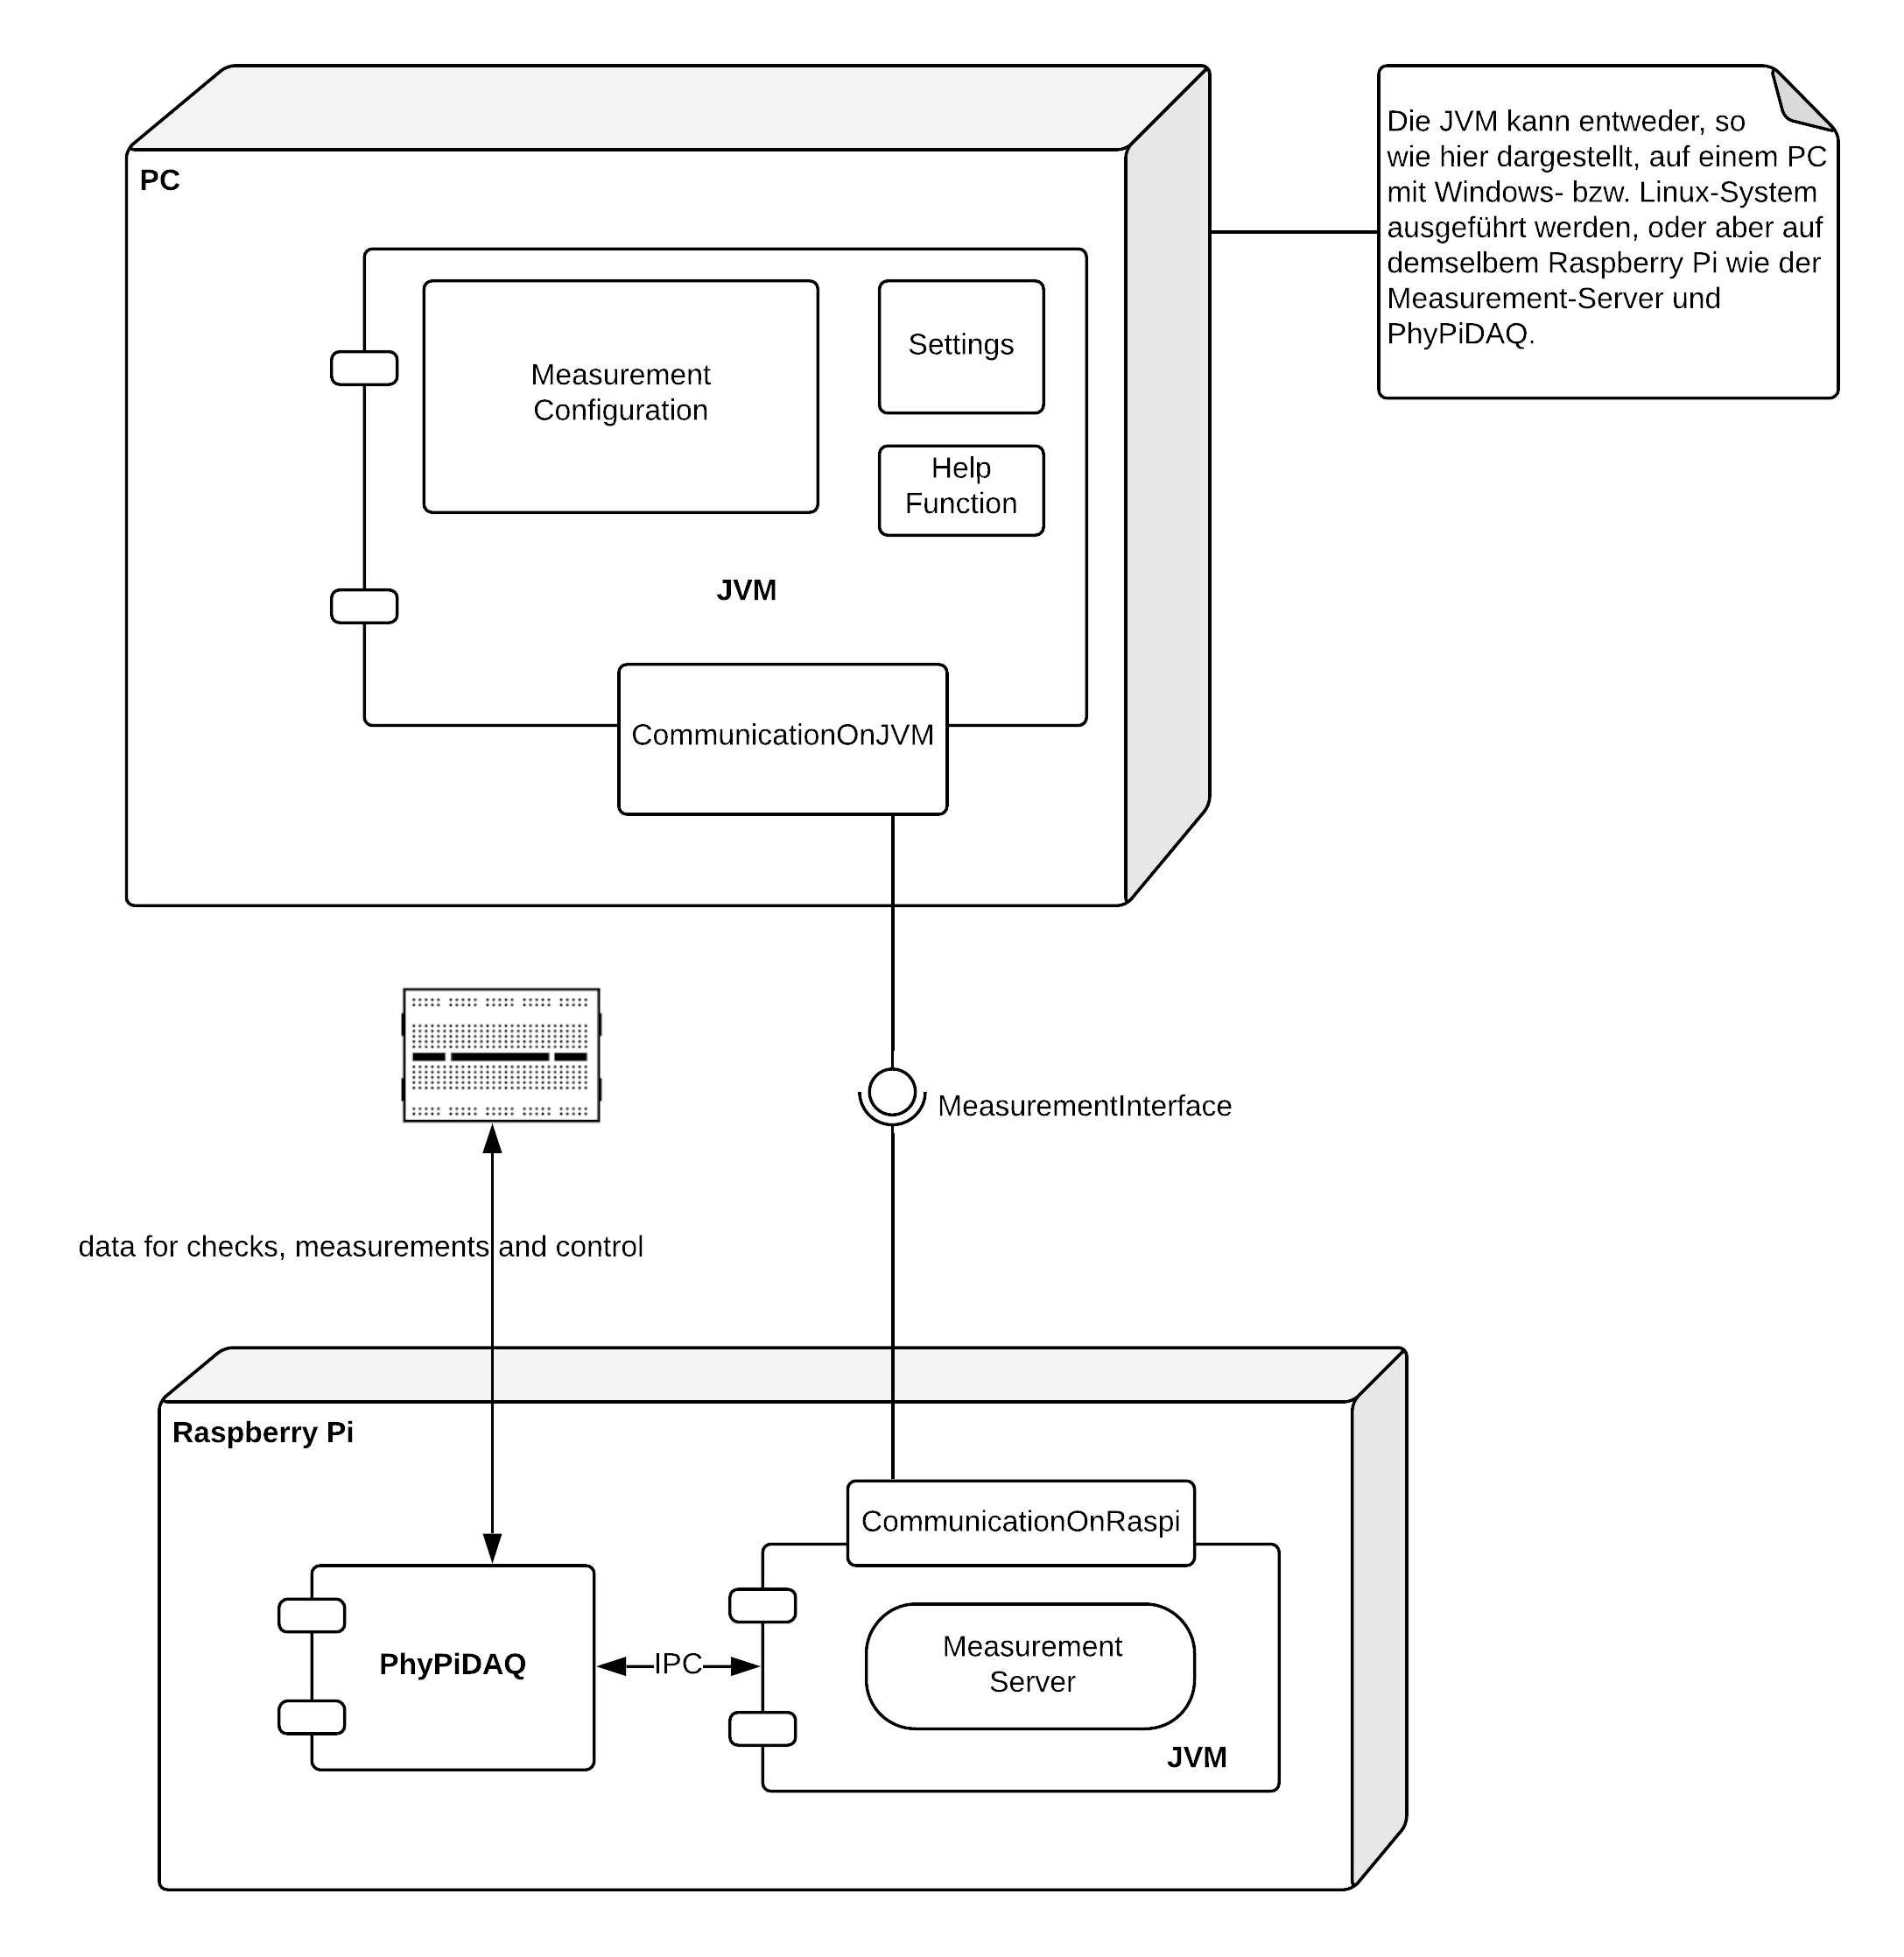
\includegraphics[width = 12cm]{Grafik/DeploymentDiagram.png}
		\caption{UML-Deployment-Diagramm}
		\label{DeploymentDiagram}
	\end{center}
\end{figure}

\section{Benutzungsoberfläche}\label{gui}

\subsection{Ziel der Benutzeroberfläche}

Das Ziel der Benutzeroberfläche ist es dem Anwender eine intuitive Benutzung des Programmes zu ermöglichen. Da das Programm im Schulbetrieb eingesetzt werden soll ist eine gute Verständlichkeit wichtig. So soll auch eine lange Einarbeitungszeit für den Anwender vermieden werden. Dabei soll keine Funktionalität verloren gehen.

\subsection{Generell}

Um die Ziele zu erfüllen wird das Programm über eine \gls{GrafBenOber}) (kurz "GUI") bedient. Der Anwender soll in der Lage sein bereits vorhandene Computer und Mobilgerät Kenntnisse zu nutzen.

\subsection{Eingabegeäte}

Die \gls{GrafBenOber} soll Maus und Tastatureingaben unterstützen. Außerdem soll eine \gls{dragdrop} Eingabe möglich sein.
Die Verwendung anderer Eingabegeräte ist nicht vorgesehen.

\subsection{Überblick}

\begin{figure}[h]
	\begin{center}
		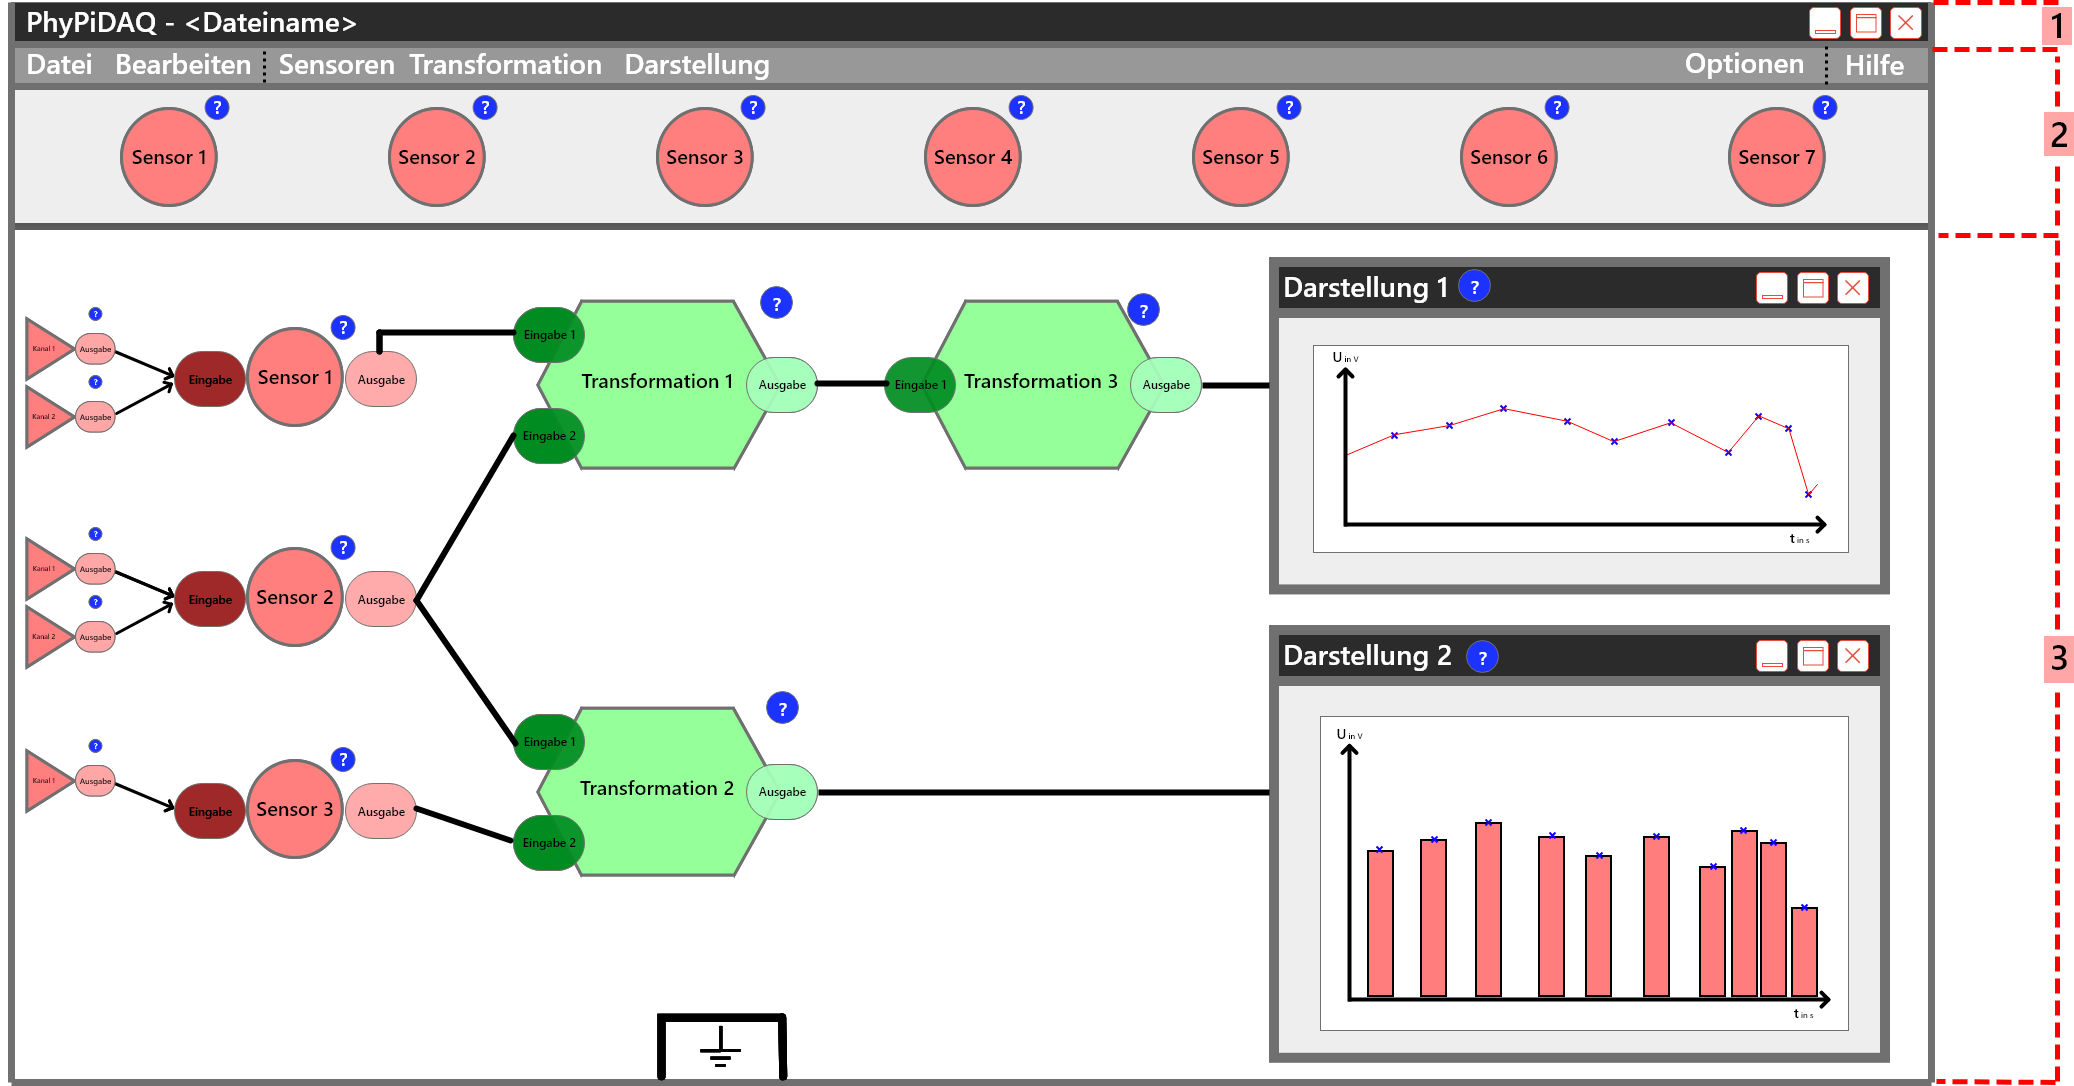
\includegraphics[width = 15cm]{Grafik/GUI-mit-Segmenten.png}
		\caption{Der Grundlegende Aufbau der Hauptbenutzeroberfläche}
		\label{GUI_Grundlage}
	\end{center}
\end{figure}

Abbildung \ref{GUI_Grundlage} zeigt den Aufbau einer möglichen \gls{GrafBenOber}. Dabei geben die Zahlen in den roten Kästchen, rechts von dem Programmfenster, die logische Unterteilung an.

Das Design der Einzelnen Elemente kann sich im Verlauf der Anwendungsentwicklung ändern. Die Grundlegenden Bausteine der \gls{GrafBenOber} werden sich in ihrer Aufgabe nicht ändern. Zu ihnen gehören:

\begin{itemize}
	\item \glspl{sensor}
	\item \glspl{transformation}
	\item \glspl{darstellung}
\end{itemize}

Die zu dem jeweiligen logischen Teil gehörenden Elemente sollen im folgenden erklärt werden.

\subsection{Die einzelnen Teile}

\subsubsection{Systemmenüleiste}
In der Systemmenüleiste befinden sich Funktionen, die Einfluss auf die gesamte \gls{GrafBenOber} haben.

\begin{tabular}[t]{p{1cm} p{10cm}} %Alle Systemmenübausteine in einer Tabelle
	\vspace{0cm}
\includegraphics[width = 1 cm]{Grafik/PhyPiDAQ.png} & Der Name des Programmes wird hier angezeigt. Rechts daneben steht, sofern vorhanden, der Name der Datei, die gerade geöffnet ist.\newline\\
	\vspace{0cm}
\includegraphics[width = 1 cm]{Grafik/Maximieren.png} & Das ''Maximieren''-Symbol vergrößert das Programmfenster auf die maximale Größe. Die Größe ist von der Benutzungsumgebung abhängig.\newline\\
	\vspace{0cm}
\includegraphics[width = 1 cm]{Grafik/Minimieren.png} & Das ''Minimieren''-Symbol blendet das Programmfenster aus. Es ist weiterhin geöffnet und wieder aufrufbar. \\
	\vspace{0cm}
\includegraphics[width = 1 cm]{Grafik/Schliessen.png} & Das ''Schliessen''-Symbol beendet die Anwendung. Vor dem Beenden findet eine Abfrage statt, ob der Anwender eventuell vorgenommene Änderungen speichern möchte.\\
\end{tabular}

\subsubsection{Auswahl}

\begin{tabular}[t]{p{1cm} p{10cm}} %Alle Auswahlelemente in einer Tabelle
	\vspace{0cm}
\includegraphics[width = 1 cm]{Grafik/Datei.png} & Der Benutzer hat die Möglichkeit Dateien zu bearbeiten. Die wichtigsten Funktionen sind:
	\begin{itemize} 
		\item Das anlegen einer neuen Datei
		\item Das Speichern der aktuellen Datei
		\item Das Öffnen einer bereits erstellten Datei
	\end{itemize}\\
	\vspace{0cm}
\includegraphics[width = 1 cm]{Grafik/Bearbeiten.png} & Der Benutzer hat die Möglichkeit den Inhalt der aktuell geöffneten Datei zu bearbeiten. Die wichtigsten Funktionen sind:
	\begin{itemize} 
		\item Das Kopieren eines ausgewählten Objektes
		\item Das Einfügen eines gespeicherten Objektes
		\item Das Anpassen eines ausgewälten Elements. Diese Einstellungsmöglichkeiten sind von dem Objekt abhängig.
	\end{itemize}\\
	\vspace{0cm}
\includegraphics[width = 1 cm]{Grafik/Sensor.png} & Der Benutzer kann sich eine Auswahl von \glspl{sensor} anzeigen lassen. Die \glspl{sensor} können anschließend in das Konfigurationsfeld eingefügt werden. Die angezeigte Auswahl ist unabhängig von den angeschlossenen Sensoren\newline\\
	\vspace{0cm}
\includegraphics[width = 1 cm]{Grafik/Verbindung.png} & Der Benutzer kann sich eine Auswahl von \glspl{transformation} anzeigen lassen. Die \glspl{transformation} können anschließend per \gls{dragdrop} in das Konfigurationsfeld gezogen werden. Die Auswahl kann unter Optionen erweitert werden.\newline\\
	\vspace{0cm}
\includegraphics[width = 1 cm]{Grafik/Darstellung.png} & Der Benutzer kann sich eine Auswahl von \glspl{darstellung} anzeigen lassen. Die \glspl{darstellung} können anschließend in das Konfigurationsfeld eingefügt werden. Die Auswahl kann erweitert werden.\newline\\
	\vspace{0cm}
\includegraphics[width = 1 cm]{Grafik/Optionen.png} & Der Benutzer kann sich eine Auswahl an Optionen anzeigen lassen. Beispiele hierfür sind
	\begin{itemize} 
		\item Das Ändern von angezeigten Farben
		\item Das Erweitern der Transformations- und Darstellungsauswahl
	\end{itemize}\\
	\vspace{0cm}
\includegraphics[width = 1 cm]{Grafik/Hilfe.png} & Der Benutzer kann sich eine allgemeine Hilfe anzeigen lassen. In der Hilfe werden die Funktionen der Anwendung erklärt.\newline\\
\end{tabular}

Im Laufe der Entwicklung kann es sich als sinnvoll herrausstellen weitere Optionen einzufügen bzw. bestehende Optionen zusammenzufügen.

\subsubsection{Konfigurationsfeld}

\begin{tabular}[t]{p{1cm} p{10cm}}
	\vspace{0cm}
\includegraphics[width = 1 cm]{Grafik/Information.png} & Das ''Informations''-Symbol zeigt nach einem Click weiterführende Informationen zu dem Element an, zu dem es gehört. So würde beispielsweise bei einer Transformation die Funktion angezeigt werde, die sie realisiert.\newline\\\cline{1-2}
	\vspace{0cm}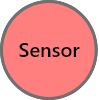
\includegraphics[width = 1 cm]{Grafik/Sensorelement.png} & Repräsentation eines Sensors, der in PhyPiDAQ erkannt werden kann. Vorraussetzung hierfür ist die Existenz einer \gls{konfigdata}.\newline\\
	\vspace{0cm}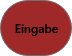
\includegraphics[width = 1 cm]{Grafik/Eingabe-Sensor.png} & Die zu einem Sensor gehörende Eingabe. Die Eingabe wird nur angezeigt, wenn auch die Kanäle angezeigt werden.\newline\\
	\vspace{0cm}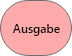
\includegraphics[width = 1 cm]{Grafik/Ausgabe-Sensor.png} & Die zu einem Sensor gehörende Ausgabe. Jeder Sensor hat genau eine Ausgabe.\newline\\
	\vspace{0cm}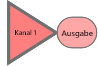
\includegraphics[width = 1 cm]{Grafik/Kanal.png} & Der zu einem Sensor gehörende Kanal. Die Anzahl an angezeigten Kanlälen hängt von dem Sensor ab. In den Optionen kann eingestellt werden, ob die Kanäle angezeigt werden.\newline\\\cline{1-2}
	\vspace{0cm}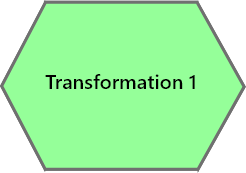
\includegraphics[width = 1 cm]{Grafik/Verbindungselement.png} & Repräsentation einer \gls{transformation}. Abhängig von der Anzahl an Eingängen der Transformation besitzt die GUI dementsprechend viele Eingänge. Jedem Eingang können durch Einfügen von einer Verbindung Daten übergegen werden.\newline\\
	\vspace{0cm}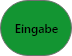
\includegraphics[width = 1 cm]{Grafik/Eingabe-Verbindung.png} & Die Eingabe einer Transformation. Die Anzahl der verfügbaren Eingaben hängt von der Transformation ab.\newline\\
	\vspace{0cm}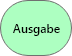
\includegraphics[width = 1 cm]{Grafik/Ausgabe-Transformation.png} & Die Ausgabe einer Transformation. Jede Transformation hat genau eine Ausgabe.\newline\\\cline{1-2}
	\vspace{0cm}
\includegraphics[width = 1 cm]{Grafik/Verbindungspfeil.png} & Eine Verbindung zwischen zwei Elementen. Sie besitz eine Richtung. Daten ''fließen'' also nicht in beide Richtungen. Sie wird durch cklicken auf zwei Elemente erstellt. Dabei ist das Element welches zuerst geclickt wurde der Anfang der Verbindung.\newline\\
\end{tabular}

\subsection{Erweiterungsmöglichkeiten}

\subsubsection{Startbildschirm}

\begin{figure}[h]
	\begin{center}
		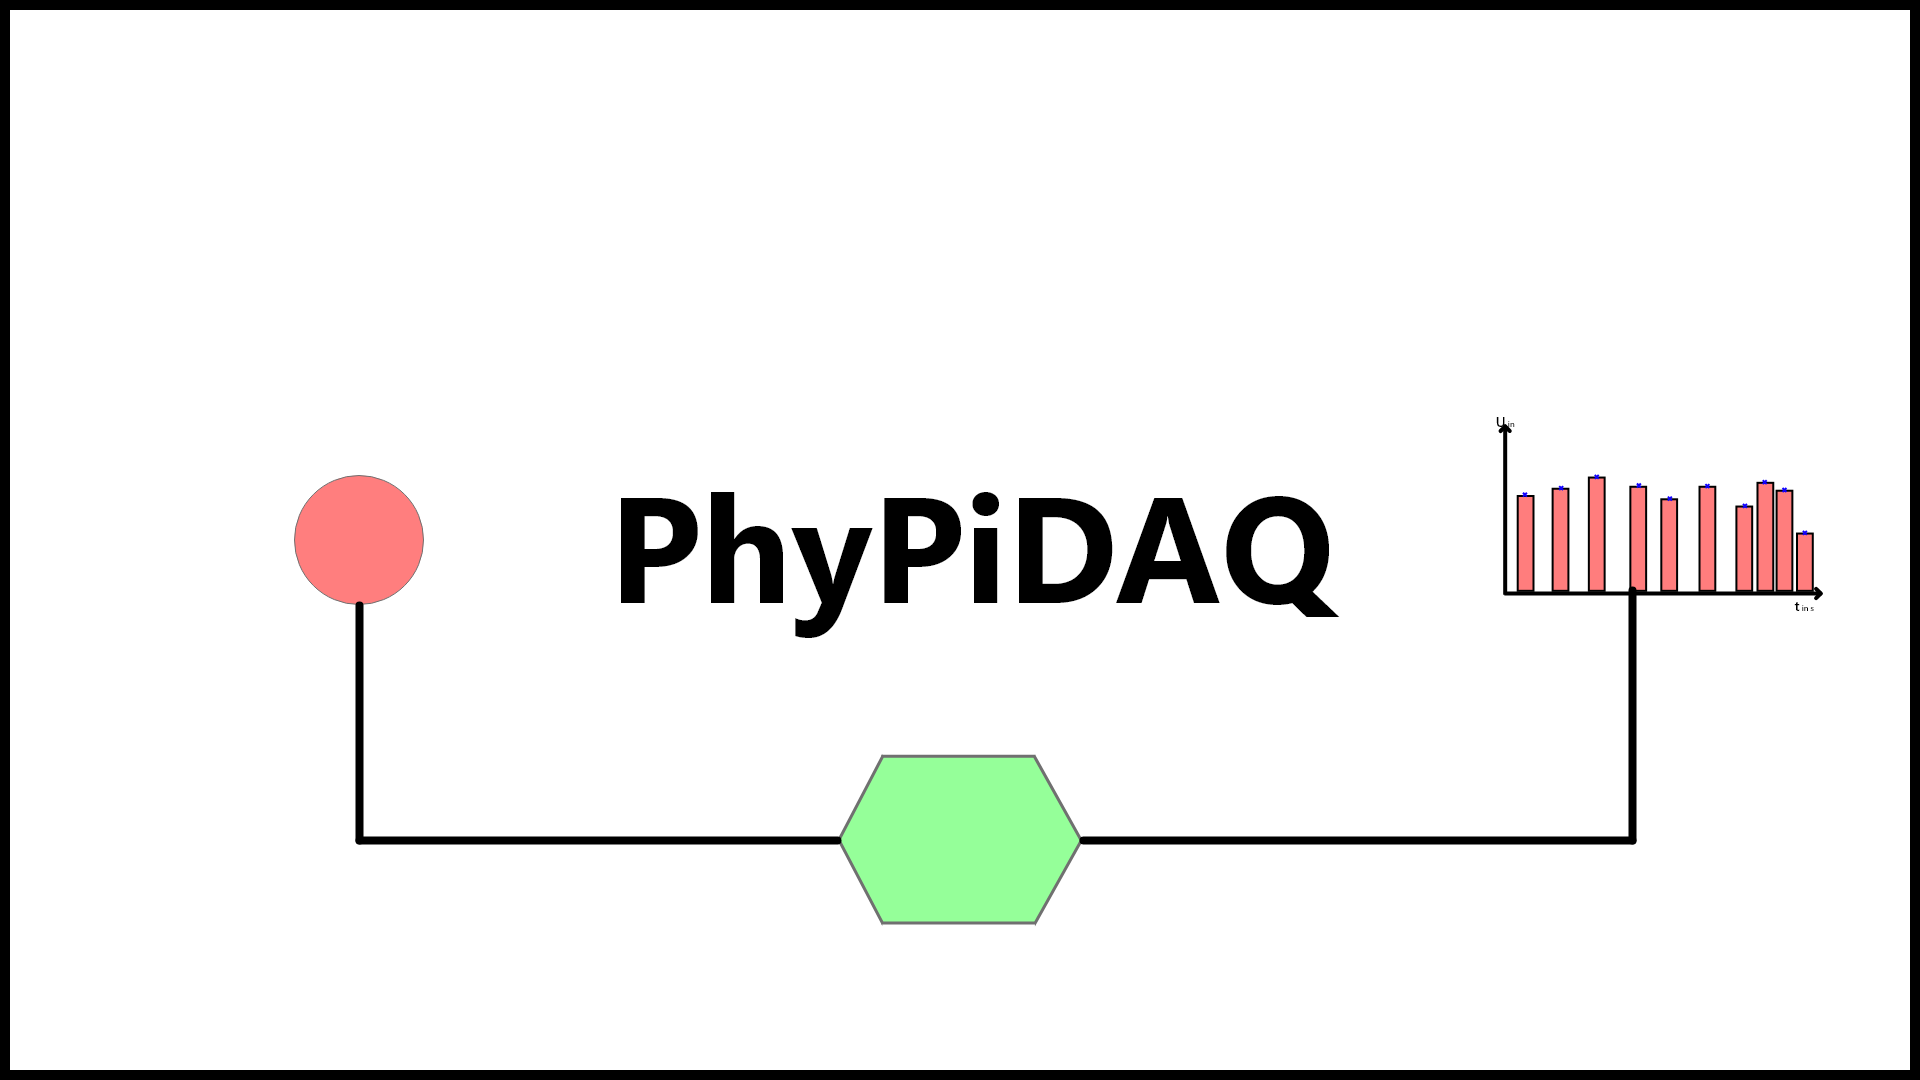
\includegraphics[width = 10cm]{Grafik/Startbildschirm.png}
		\caption{Ein Beispiel für einen Startbildschirm}
		\label{startbildschirm}
	\end{center}
\end{figure}

Eine Erweiterungsmöglichkeit wäre das Einfügen eines Startbildschirmes vor dem Öffnen der Anwendung. Dieser ist in Abbildung \ref{startbildschirm} angedeutet.

\section{Spezielle Anforderungen an die Entwicklungsumgebung}\label{entwicklungsumgebung}

Für die Umsetzung des Projekts ist Zugang zu funktionierender Hardware (kontret: mindestens ein \gls{RasPi}, möglichst mehrere \glspl{sensor}, Peripheriegeräte) notwendig, um die Funktionalität des Produkts sicherzustellen.\newline
Ansonsten muss gegebenenfalls auf simulierte \gls{messdaten} zurückgegriffen werden.

\section{Zeit- und Ressourcenplanung}\label{zeit}

\subsection{Projektphasen}

\begin{tabular}{| l | l | l | r |}
	\hline
	\textbf{Phase} & \textbf{Verantwortlicher} & \textbf{Zeitraum} & \textbf{Kolloquium} \\ \hline
	Pflichtenheft & Jan Küblbeck & KW 20–22 & 04.06.2019 \\
	Entwurf & Leon Huck & KW 23–26 & 02.07.2019 \\
	Implementierung & Stefan Geretschläger & KW 27–29, 31 & (tbd) \\
	Klausurenphase & — & KW 30, 32 & — \\
	Qualitätssicherung & David Gawron & KW 33–35 & 03.09.2019 \\
	Abnahme & — & KW 36 & — \\
	Abschlussprüfung & Linus Ruhnke & KW 37/38 & (tbd) \\
	\hline
\end{tabular}

\subsection{Risikomanagement}

In jeder Phase treten unterschiedliche Risiken auf.

Das Ausfallen eines Teammitglieds durch Krankheit oder andere Gründe ist ein bedeutendes Risiko. In diesem Fall muss die zusätzliche Arbeit gerecht auf die anderen Teilnehmer verteilt werden. Eventuell können dadurch einzelne Kriterien und Anforderungen nicht mehr zufriedenstellend erfüllt werden.

\section{Ergänzungen}\label{erweiterung}

\section{Glossar}\label{glossar}

\renewcommand*{\glossarysection}[2][]{}	% prevents double glossary section heading
\printnoidxglossaries				% generate pdf twice when adding new entries


\end{document}\grid
